\documentclass[12pt]{article}
\usepackage[margin=1in]{geometry}
\usepackage{amsmath}
\usepackage{graphicx}
\usepackage{setspace}
\usepackage{subcaption}
\usepackage{listings}
\usepackage[italicdiff]{physics}
\usepackage{natbib}
\usepackage{epstopdf}
\lstset{breaklines=true, tabsize = 3}

\author{Jonathan Bunton}
\title{Modeling Atomic Interactions in Xenon \\ Using the Morse and Lennard-Jones Potentials}
\date{\today}

\begin{document}
\maketitle
\onehalfspacing
\begin{abstract}
Several models exist for inter-atomic forces, the majority of which with the basis of weak attractive force at long range, countered by a strong repulsive force at close distance.    Two such models are the Lennard-Jones and Morse potentials, each of which accomplish this behavior with differing mathematical models.  

This paper analyzes the behavior of a lattice of Xenon atoms in both the Lennard-Jones and the Morse potentials by using Verlet integration to simulate atomic behavior using parameters for these potentials as experimentally determined from the second virial coefficient. \cite{mconstants, ljconstants}  Verlet integration shows excellent conservation of momentum and energy, with a maximum deviation on the order of 0.01\%.\cite{verlet}  The data also exhibits the spring-esque behavior suggested by the potential curves, with the Morse potential ultimately showing a more oscillatory behavior due to its more flexible parameters.  In addition, both potentials exhibit evaporation and decreased order with increased temperature.
\end{abstract}

\section*{Introduction}
Various mathematical models exist to approximate the shape of inter-atomic potentials.  The fundamental idea behind each is to accurately represent both the attractive long-range forces and the repulsive short-range forces within the same model.  Two of the most popular models for these interactions (which behave particularly well in the case of noble gases) are the Lennard-Jones and Morse potentials.  Both potentials are characterized by a well-shaped curve, with various parameters to control the shape, which are dependent on the element at hand.

The Lennard-Jones potential is generally nicknamed the ``6-12" potential, as it achieves the well-shaped potential behavior by using negative powers of $r$, shown in eq. \ref{LJpot}. The Lennard-Jones potential creates this with two terms:
\begin{equation}
\label{LJpot}
U(r) = \varepsilon\left[ \left( \frac{r_m}{r} \right)^{12}-2\left(\frac{r_m}{r}\right)^6\right]
\end{equation}
Here $r$ is the distance between particles, and the parameters $\varepsilon$ and $r_m$ determine the depth of the potential curve and its lowest point, respectively. \cite{ljpotential} The parameters $\epsilon$ and $r_m$ are determined both computationally and experimentally, generally being derived from the second virial coefficient. \cite{ljconstants} The Morse potential achieves a similar shape with a different mathematical approach:
\begin{equation}
\label{morsepot}
U(r) = D_e \left(1-e^{-a(r-r_e)}\right)^2
\end{equation}
In this potential, the parameters $D_e$ and $a$ control the depth and width of the potential well, while $r_e$ is the lowest point. \cite{mpotential}  The inclusion of three parameters rather than the two in the Lennard-Jones potential gives the Morse potential more control over the well depth and width.  These parameters are also often derived from a combination of computational and experimental methods. \cite{mconstants}

Both of these potentials can then be used to calculate conservative forces between two or more particles.  The system in question in this paper is a lattice of Xenon atoms, with lattice spacing such that the system is in a relatively low potential energy state.  Due to the shape of both potentials, this defines lattices with $r_m$ spacing for the Lennard-Jones potential and $r_e$ spacing in the Morse potential.

Because these potentials produce conservative vector fields, the fundamental conservation laws hold for the system of atoms.  This means that as a measure of numerical accuracy, the linear momentum, angular momentum, and energy in the system should remain constant throughout.  The linear momentum of the system (and therefore the linear momentum in each direction) must be constant, as well as the total energy, in order for the simulation to be considered accurate.  This motivates the monitoring and plotting of these values over time, as shown below.

The simulation as a whole hinges on the initialization of a lattice of Xenon atoms, generation of initial velocities for each particle, and the calculation of the positions of each particle over time within a position-based potential function, all the while keeping total momentum and energy constant throughout.  This paper does all this through the use of Verlet integration as a method of inteagral approximation with discrete timesteps.

\section*{Methods}
The Fortran code written to model this system uses Velocity Verlet, which is based on Verlet integration within a position-based potential.  Recalling the equations of motion for a conservative system,  $\vec{F} = m\vec{a}(t) = -\nabla V(\vec{r}(t)),$ it is clear that within the discrete system, the negative gradient of the potential function will need to be recalculated at each time step.  If this force is assumed roughly constant within the time step considered, the equations of motion are then:
\begin{align}
\vec{v}(t) &= \vec{v}(0) + \frac{1}{2}\vec{a}(t) \\
\vec{r}(t) &= \vec{r}(0) + \vec{v}(t) + \frac{1}{2}\vec{a}(t)^2 
\end{align}
Verlet integration, or in this case the nicknamed algorithm Velocity Verlet, uses a central difference approximation to the second derivative to provide a value for the acceleration at a given point.  Utilizing Velocity Verlet also requires a discretization of the system in time, where the equations of motion are instead calculated with a discrete timestep $\Delta t$ to yield:
\begin{align}
\vec{v}(t+\Delta t) &= \vec{v}(t) + \frac{\vec{a}(t) + \vec{a}(t+\Delta t)}{2}\Delta t \\
\vec{r}(t+\Delta t) &= \vec{r}(t) + \vec{v}(t)\Delta t + \frac{1}{2}\vec{a}(t)\Delta t^2
\end{align}
This set of discrete equations indicates that at each time step, calculating forward a single timestep requires calculating the value of the acceleration at the current time, using the negative gradient of the potential.  Because the Morse and Lennard-Jones potentials depend on the relative positions of particles with respect to each other, each timestep requires calculations of the force (and therefore acceleration) from each particle in the system, added together in a vector sum.  Once the accelerations have been calculated at the current time $t$, the velocity followed by the position at time $t + \Delta t$ can be found for each particle in the system.  This algorithm repeats recursively for as many timesteps forward as required for the time interval considered.

This algorithm is simple, but requires an initial velocity condition for the system.  To maintain a realistic model, the velocities are sampled from the Maxwell velocity distribution in each dimension $i$ that is dependent on the temperature of the molecules within the system:
\begin{align}
f_v(v_i) &= \sqrt{\frac{m}{2\pi k T}}\exp\left(\frac{-mv_i^2}{2kT}\right),
\end{align}  where $m$ is the particle's mass and $k$ is Boltzmann's constant.  This distribution allows for realistic temperature-dependent behavior within the system, which is evident based on the results shown below.  To generate velocities from this distribution, it is worth noting that the Maxwell distribution is simply a normal distribution with mean $\mu = 0$ and a standard deviation $\sigma = \sqrt{\frac{kT}{m}}$.  For convenience, this could be brought to the standard normal distribution with a z-transform $z = \frac{v}{\sigma}$.  Because Fortran will only generate random numbers on the unit interval, the use of a Box-Muller transform is convenient. \cite{boxmuller}  The Box-Muller transform takes numbers $U_1, U_2$  from a uniform distribution and transforms them to numbers from the standard normal distribution through the equations:
\begin{align}
Z_1 &= \sqrt{-2\ln U_1}\cos(2\pi U_2) \\
Z_2 &= \sqrt{-2\ln U_1}\sin(2\pi U_2).
\end{align}
Considering an initial z-transform, to generate random numbers from the Maxwell distribution from random uniformly distributed numbers $U_1, U_2$:
\begin{align}
v_1 & = \sqrt{\frac{-2m\ln(U_1)}{kT}}\cos(2\pi U_2) \\
v_2 & = \sqrt{\frac{-2m\ln(U_1)}{kT}}\sin(2\pi U_2).
\end{align}

These velocities are initialized alongside the lattice position at the start of the program, which then undergoes 1000 time steps of $\Delta t = 10^{-14}$ seconds.  Because of the dependence on temperature, several simulations were performed with various temperature conditions to reveal some temperature-dependent behaviors inherent in the system.

\section*{Results}
Both the Lennard-Jones and Morse potentials were simulated using a Fortran code.  In order to provide the most realistic system, the code initializes the velocities in each direction using the Maxwell-Boltzmann distribution in each dimension.  The system proved semi-stable for both cases, with a slight oscillatory behavior as expected from the potential shapes.  Ultimately, the steady-state solution appeared to be a sphere, where each particle is spaced at an adequate distance to be ``trapped" in the curve of the potential well.
\subsection*{Lennard-Jones Potential}
The Lennard-Jones (6-12) potential creates a semi-stable system.  Our simulation remains stable throughout the movement of the atoms, provided a small enough time-step, in this case $10^{-14}$ seconds.  This is shown most clearly by the stability of the graphs in figs. \ref{LJEconservation} and \ref{LJPconservation}, which  exhibit a deviation on the order of 0.01\% in total energy and $<$ 0.01\% in total momentum.  This is expected in an acceptable model for the system, proving Verlet integration as a viable method of calculation in this code.  These percentages hold for timesteps of $10^{-14}$, but smaller timesteps provide more accuracy.  Conversely, larger timesteps result in too drastic of changes in the system for momentum and energy to be effectively conserved.

%L-J CONSERVATION PICS
\begin{figure}[!h]
\begin{subfigure}{0.5\textwidth}
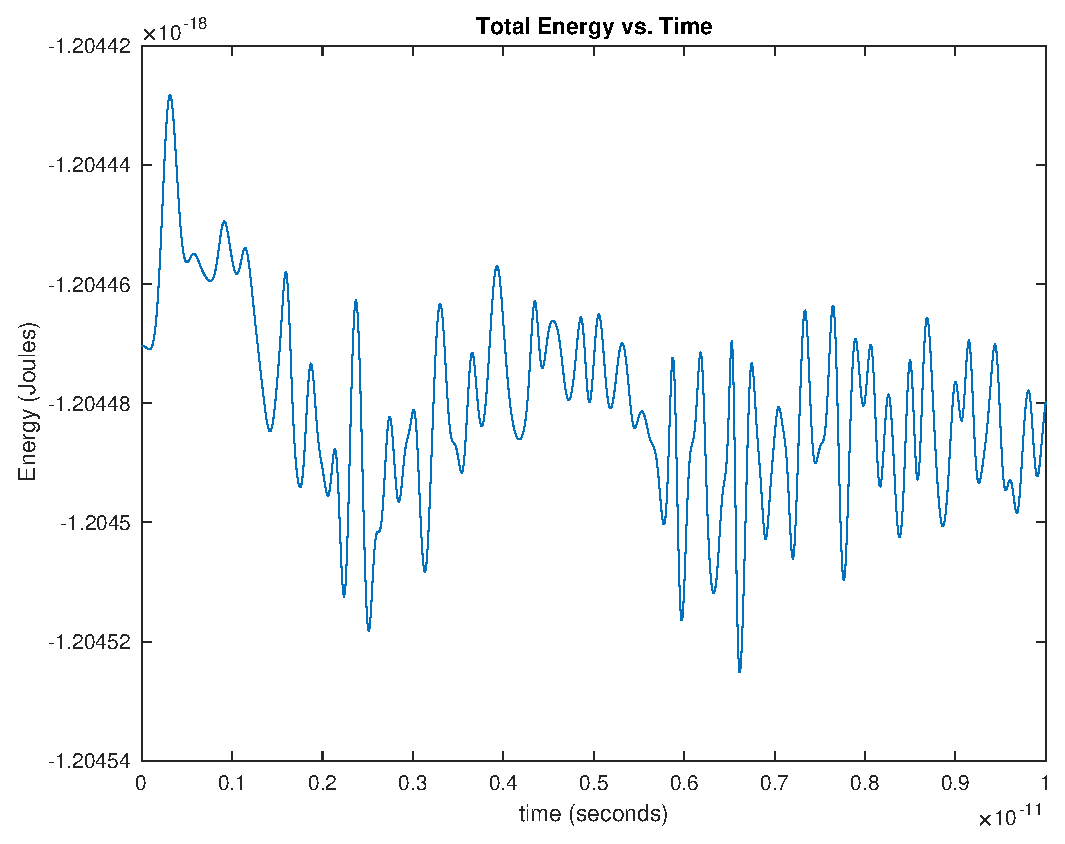
\includegraphics[width=0.9\linewidth]{./finalpics/LJEvsT.eps}
\caption{\label{LJEconservation}}
\end{subfigure}
\begin{subfigure}{0.5\textwidth}
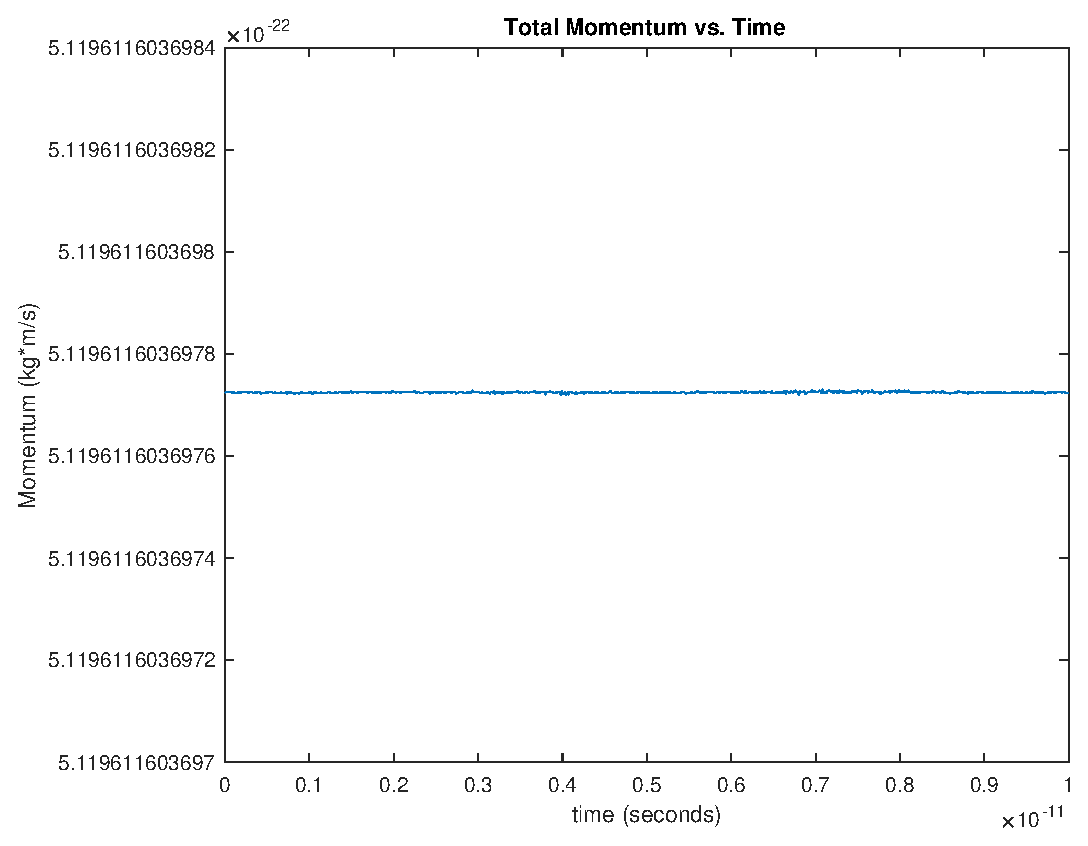
\includegraphics[width=0.9\linewidth]{./finalpics/LJPvsT.eps}
\caption{\label{LJPconservation}}
\end{subfigure}
\caption{Plots of (a) total system energy, and (b) total momentum magnitude vs. time for a lattice of Xenon atoms in the Lennard-Jones potential.  These graphs were simulated with a temperature of 100K.  The extremely stable results show that there is only a variation in energy on the order of 0.01\% and $<$ 0.01\% for momentum.} 
\end{figure} 

Shifting instead to the resulting position data, the initial and final states of the system are shown in figs. \ref{LJinitial} and \ref{LJfinal}.  In this potential, the atoms are initialized to a lower velocity due to the low temperature, and thus behave similarly to if they were to begin with zero velocity.  In this situation, each atom is at a minimum $r_e$ distance apart, causing the long-range attractive force to dominate.  After this attractive force acts on the particles, the atoms move closer and experience the abrupt short-range repulsive forces.  This causes a slight contraction-expansion cycle as the atoms readjust to a more energetically favorable position.  This is visualized through the plot in fig. \ref{LJaverager}, where the average displacement magnitude shows slight signs of oscillation over time.

%L-J INITIAL AND FINAL SCATTERS
\begin{figure}[!h]
\begin{subfigure}{0.5\textwidth}
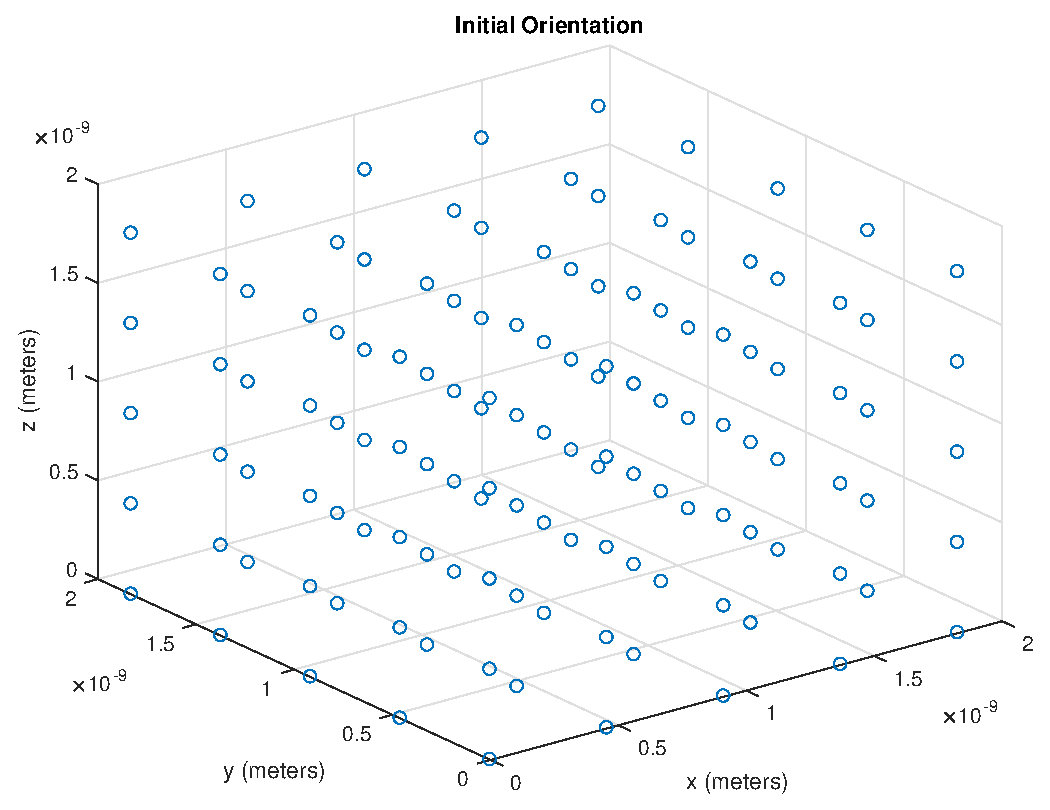
\includegraphics[width=0.9\linewidth]{./finalpics/LJinitial.eps}
\caption{\label{LJinitial}}
\end{subfigure}
\begin{subfigure}{0.5\textwidth}
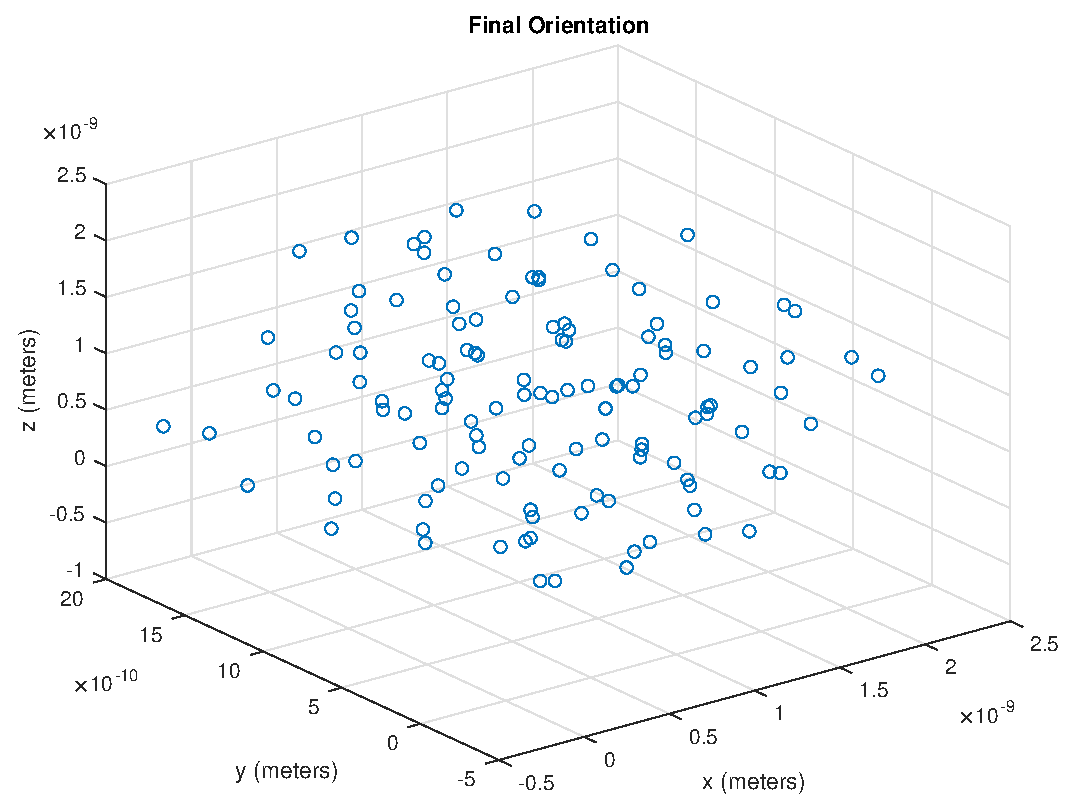
\includegraphics[width=0.9\linewidth]{./finalpics/LJfinal.eps}
\caption{\label{LJfinal}}
\end{subfigure}
\caption{3D scatter plots of (a) initial system position, and (b) final system position for Xenon atoms in the Lennard-Jones potential.  These graphs were simulated with a temperature of 100K.  The system shifts from a lattice to a more energetically favorable spherical shape, as expected when below its boiling point.} 
\end{figure}

%L-J AVERAGE DISPLACEMENT
\begin{figure}
\begin{center}
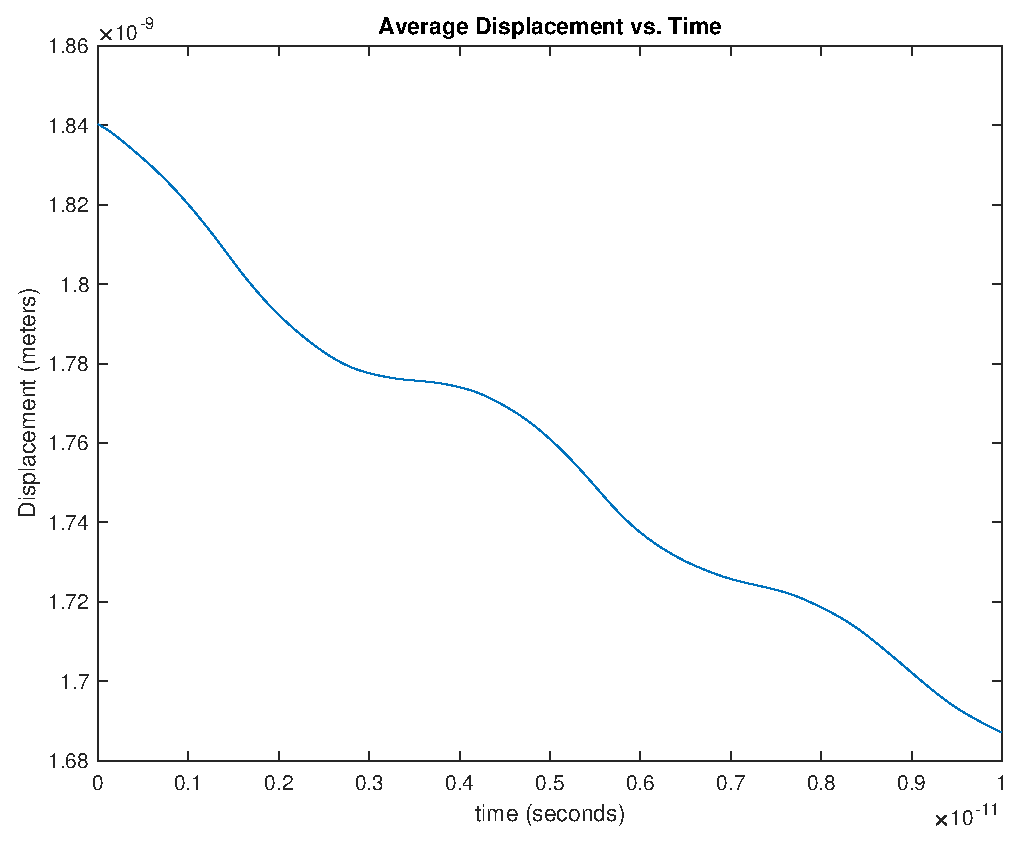
\includegraphics[width=0.5\textwidth]{./finalpics/LJaverager.eps}
\caption{\label{LJaverager} A plot of the average magnitude of the displacement from the origin over time for Xenon atoms in the Lennard-Jones potential.  As the atoms repeatedly expand and contract, there is a definite trend in the average displacement magnitude as it increases and decreases.  It appears to stabilize over time, but trend slightly closer to the origin as the particles arrange themselves more spherically (and therefore closer to the axes' origin).}
\end{center}
\end{figure}

\subsection*{Morse Potential}
In the Morse potential, the oscillatory behavior within the potential is again very evident.  The energy and momentum of the system are conserved with comparable accuracy on the order of $<$ 0.01\%, as seen in figs \ref{MEconservation} and \ref{MPconservation}.  This once again validates the use of Verlet integration to simulate this system, provided an appropriate time step is used for the potential.

%MORSE CONSERVATIONS
\begin{figure}[!h]
\begin{subfigure}{0.5\textwidth}
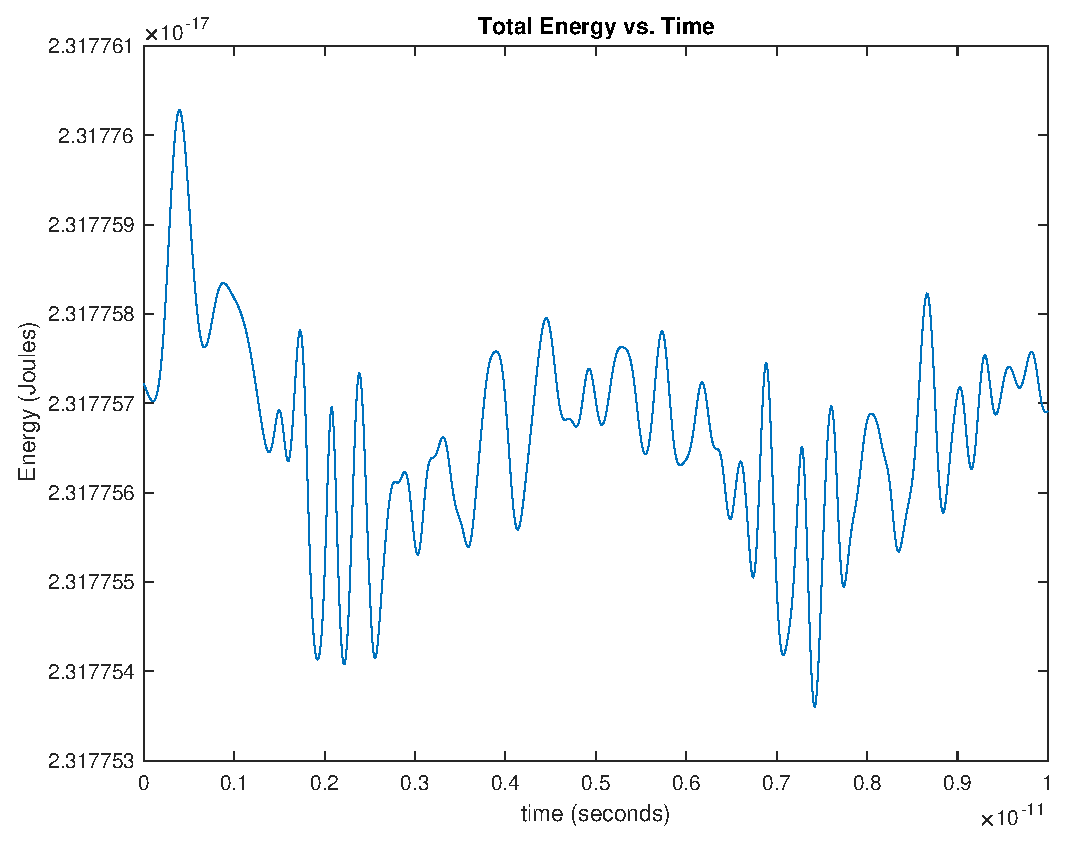
\includegraphics[width=0.9\linewidth]{./finalpics/MEvsT.eps}
\caption{\label{MEconservation}}
\end{subfigure}
\begin{subfigure}{0.5\textwidth}
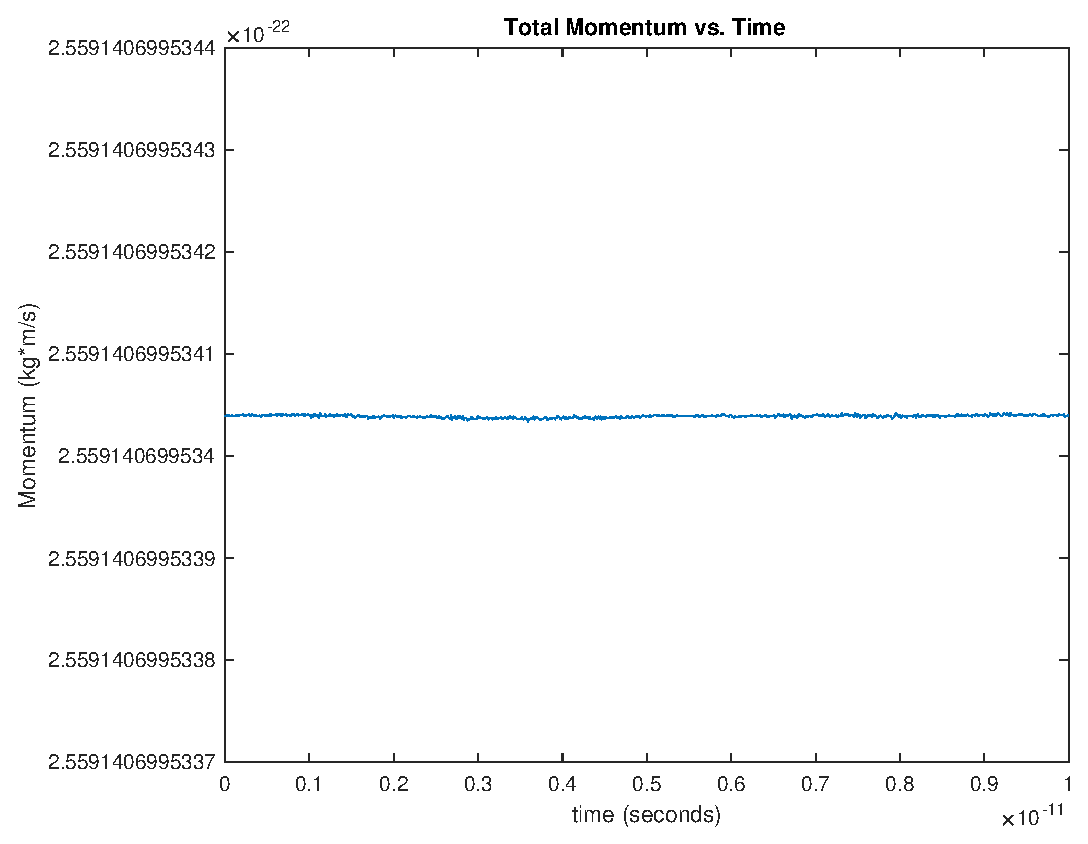
\includegraphics[width=0.9\linewidth]{./finalpics/MPvsT.eps}
\caption{\label{MPconservation}}
\end{subfigure}
\caption{Plots of (a) total system energy, and (b) total momentum magnitude vs. time for a lattice of Xenon atoms in the Morse potential.  These graphs were simulated with a temperature of 100K.  The extremely stable results show that there is a variation $<$ 0.01\% for both energy and momentum.} 
\end{figure}

After validating the model through acceptable conserved quantities, the results of the Morse potential are very similar to those in the Lennard-Jones.  Because each atom is initialied at a minimum distance $r_m$ from its neighbors, the long-range attractive force dominates.  As this force pulls the atoms inward, the short-range repulsive force acts, causing a nearly identical contraction-expansion cycle to that seen in the Lennard-Jones potential.  The Morse potential, however, exhibits noticeably larger oscillations, perhaps owed somewhat to the flexibility in the width parameter $a$ that does not exist in the Lennard-Jones.  This pattern is shown in fig. \ref{Maverager}, which displays heavy oscillations in the average magnitude of the displacement.

%MORSE INITIAL AND FINAL SCATTERS
\begin{figure}[!h]
\begin{subfigure}{0.5\textwidth}
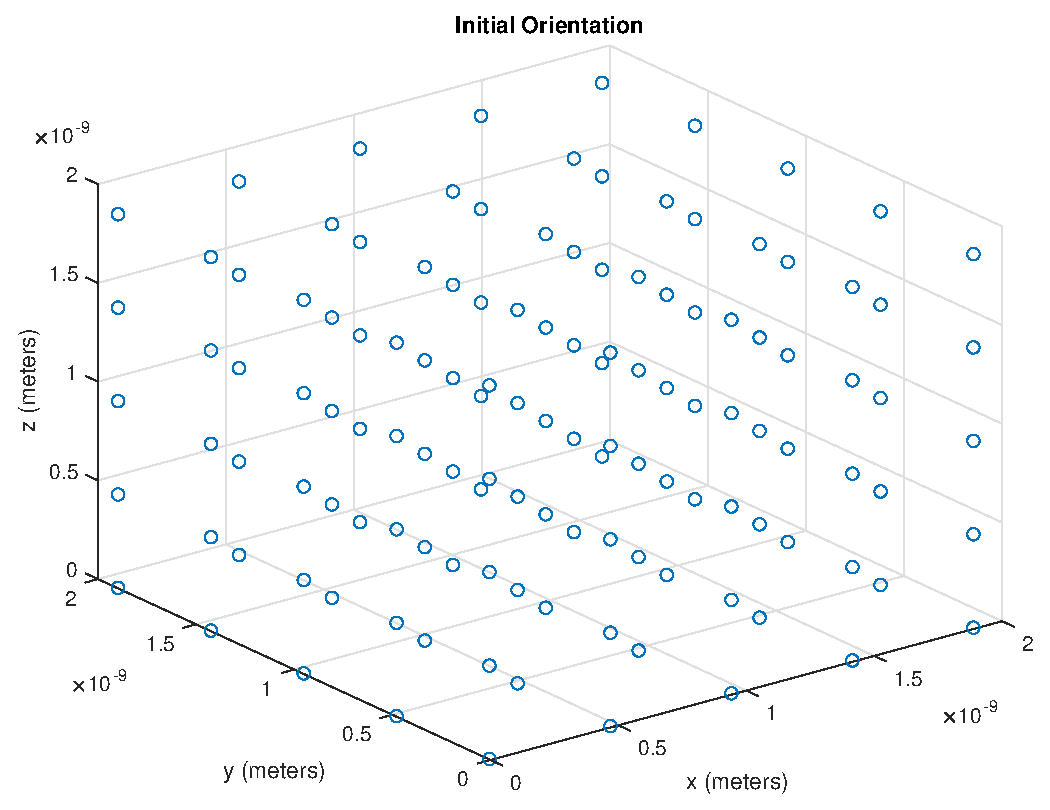
\includegraphics[width=0.9\linewidth]{./finalpics/Minitial.eps}
\caption{\label{Minitial}}
\end{subfigure}
\begin{subfigure}{0.5\textwidth}
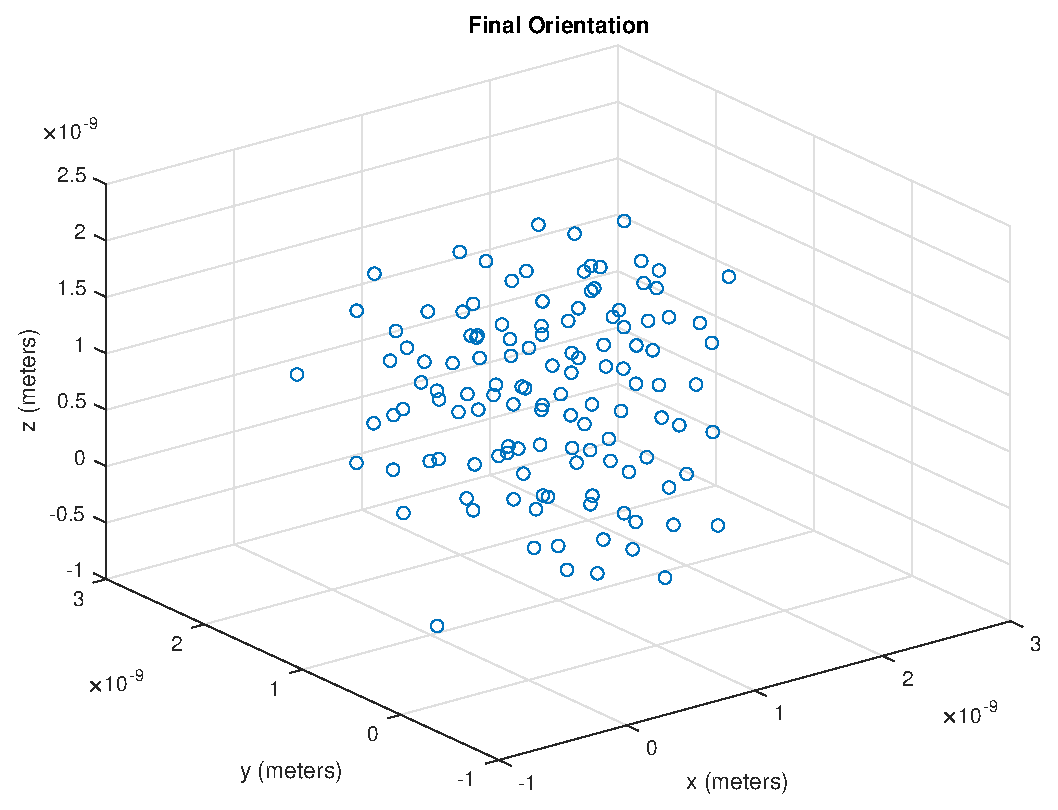
\includegraphics[width=0.9\linewidth]{./finalpics/Mfinal.eps}
\caption{\label{Mfinal}}
\end{subfigure}
\caption{3D scatter plots of (a) initial system position, and (b) final system position.  These graphs were simulated with a temperature of 100K.  The system shifts from a lattice to a more energetically favorable spherical shape, as expected when below its boiling point.} 
\end{figure}

In addition to the oscillatory behavior shown in fig. \ref{Maverager}, the 3D scatter plots in figs. \ref{Minitial} and \ref{Mfinal} show that the Morse potential tends to pull particles slightly closer together than the Lennard-Jones.  Because the Morse potential has more control over the potential well width, this is somewhat expected.

%MORSE AVERAGE DISPLACEMENT
\begin{figure}
\begin{center}
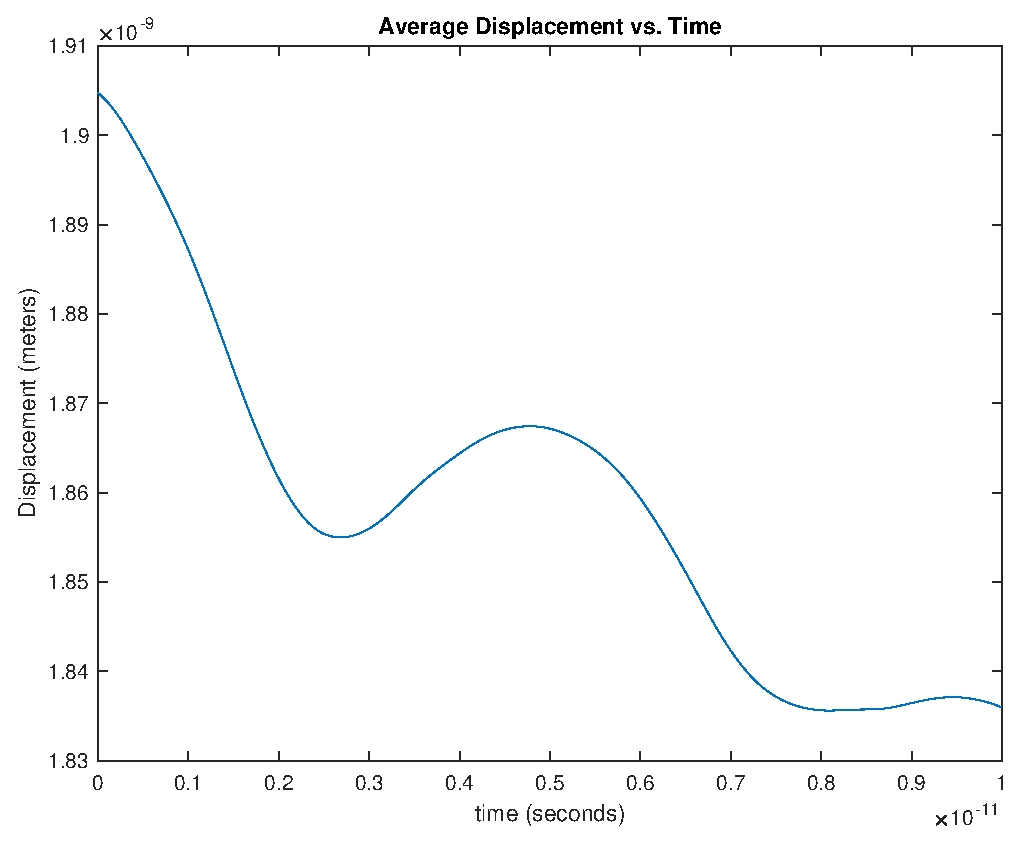
\includegraphics[width=0.5\textwidth]{./finalpics/Maverager.eps}
\caption{\label{Maverager} A plot of the average magnitude of the displacement from the origin over time for Xenon atoms in the Morse potential.  As was seen in the Lennard-Jones potential, the atoms repeatedly expand and contract, creating a trend in the average displacement magnitude.  It appears to stabilize over time, but trend slightly closer to the origin as the particles arrange themselves more spherically (and therefore closer to the axes' origin).}
\end{center}
\end{figure}
\subsection*{Temperature Considerations}
In both potentials, the initial velocity in each direction for each atom was drawn from the Maxwell velocity distribution.  This distribution inherently depends on temperature, and therefore as we increase the temperature, the standard deviation of our initial velocity also increases (see figs. \ref{maxwell100} and \ref{maxwell1000}).  This is to be expected, as the Maxwell velocity distribution is merely a normal distribution with $\mu = 0$ and $\sigma = \sqrt{\frac{K_bT}{m}}$.

%SAMPLING DISTRIBUTIONS
\begin{figure}[!h]
\begin{subfigure}{0.5\textwidth}
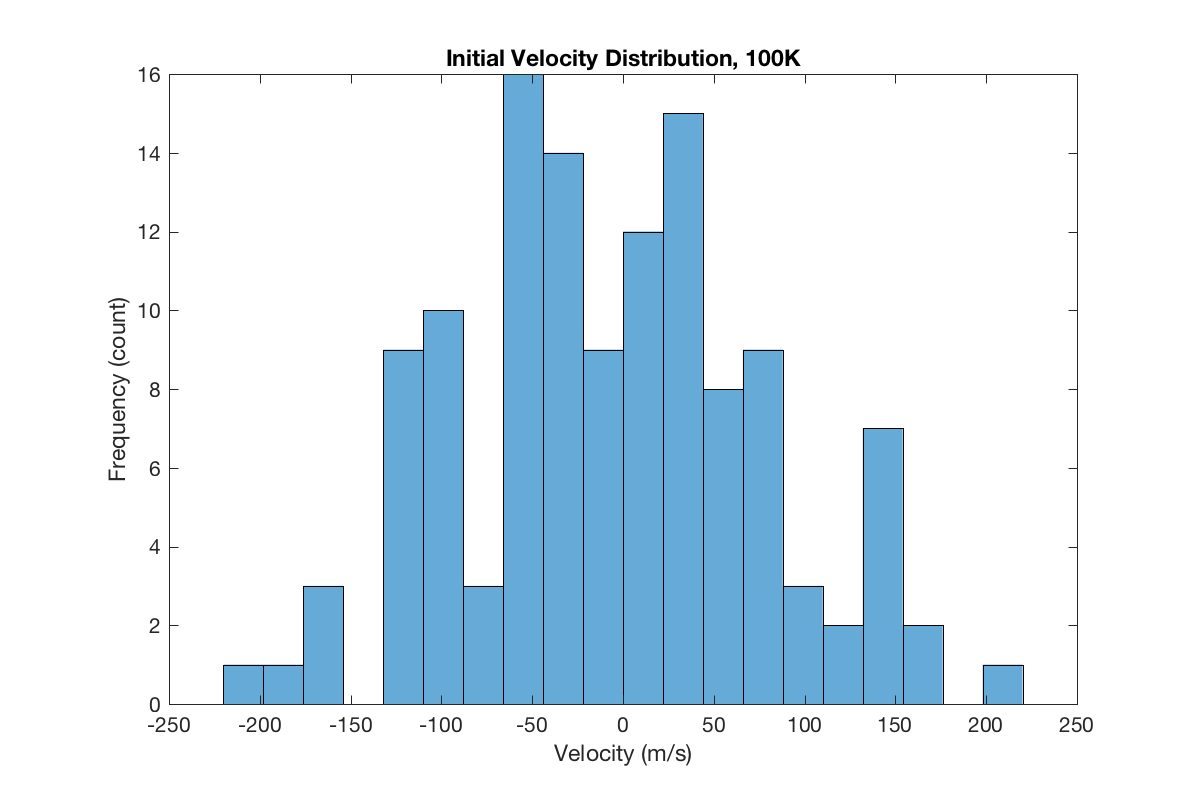
\includegraphics[width=\linewidth]{./finalpics/100initialvelocity.eps}
\caption{\label{maxwell100}}
\end{subfigure}
\begin{subfigure}{0.5\textwidth}
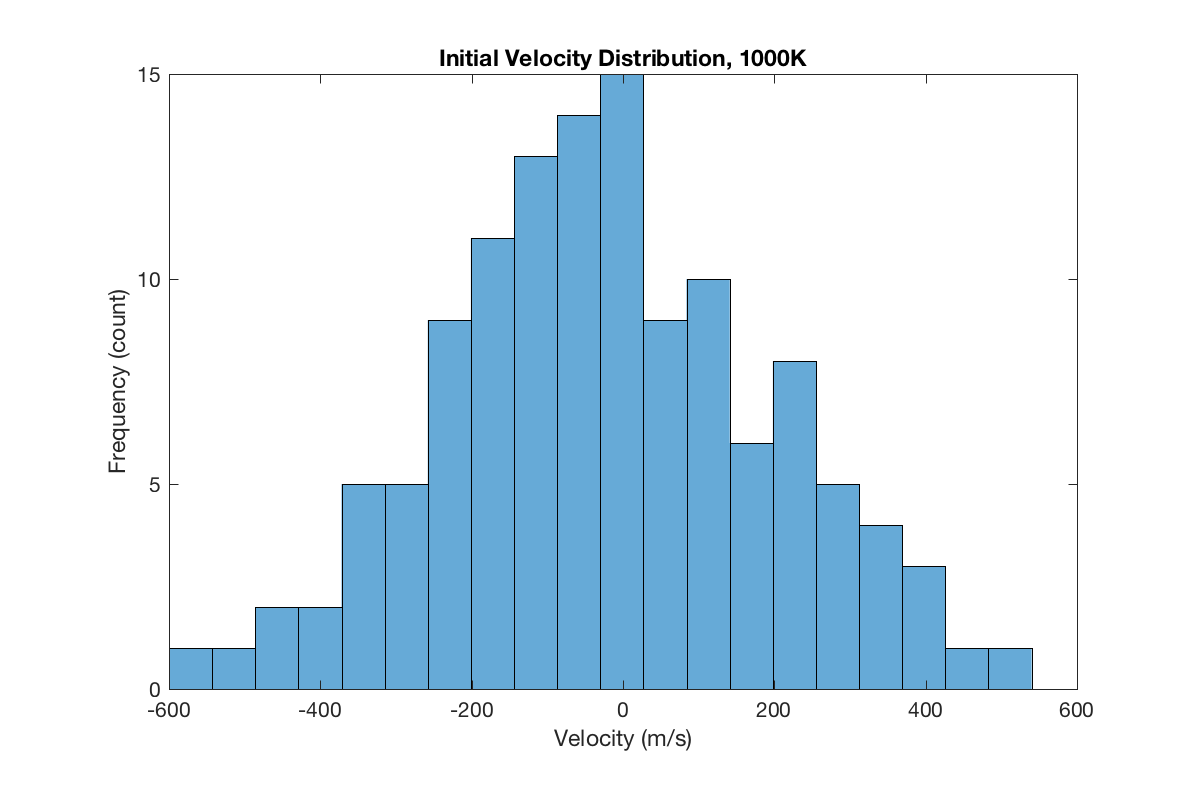
\includegraphics[width=\linewidth]{./finalpics/1000initialvelocity.eps}
\caption{\label{maxwell1000}}
\end{subfigure}
\caption{Histograms displaying the initial distributions of the initial x-component of the velocity at (a) 100K and (b) 1000K.  These distributions are similar in shape, but as the temperature increases, the atoms are permitted to move faster initially.  This higher initial velocity causes more evaporation of atoms.} 
\end{figure}
The direct result of this distribution is the evaporation of more atoms in the system, as shown in the figs. \ref{LJfinal1000}, \ref{LJaverage1000}, \ref{Mfinal1000}, and \ref{Maverage1000}.  The upward trend in the average displacement indicates a trend of general evaporation upon initialization, where some atoms are initialized with enough energy to effectively escape the long-range attractive force of the other atoms in the system.  This happens regardless of potential, although the Morse potential appears to exhibit evaporation at a slightly faster rate.

\begin{figure}[!h]
\begin{subfigure}{0.5\textwidth}
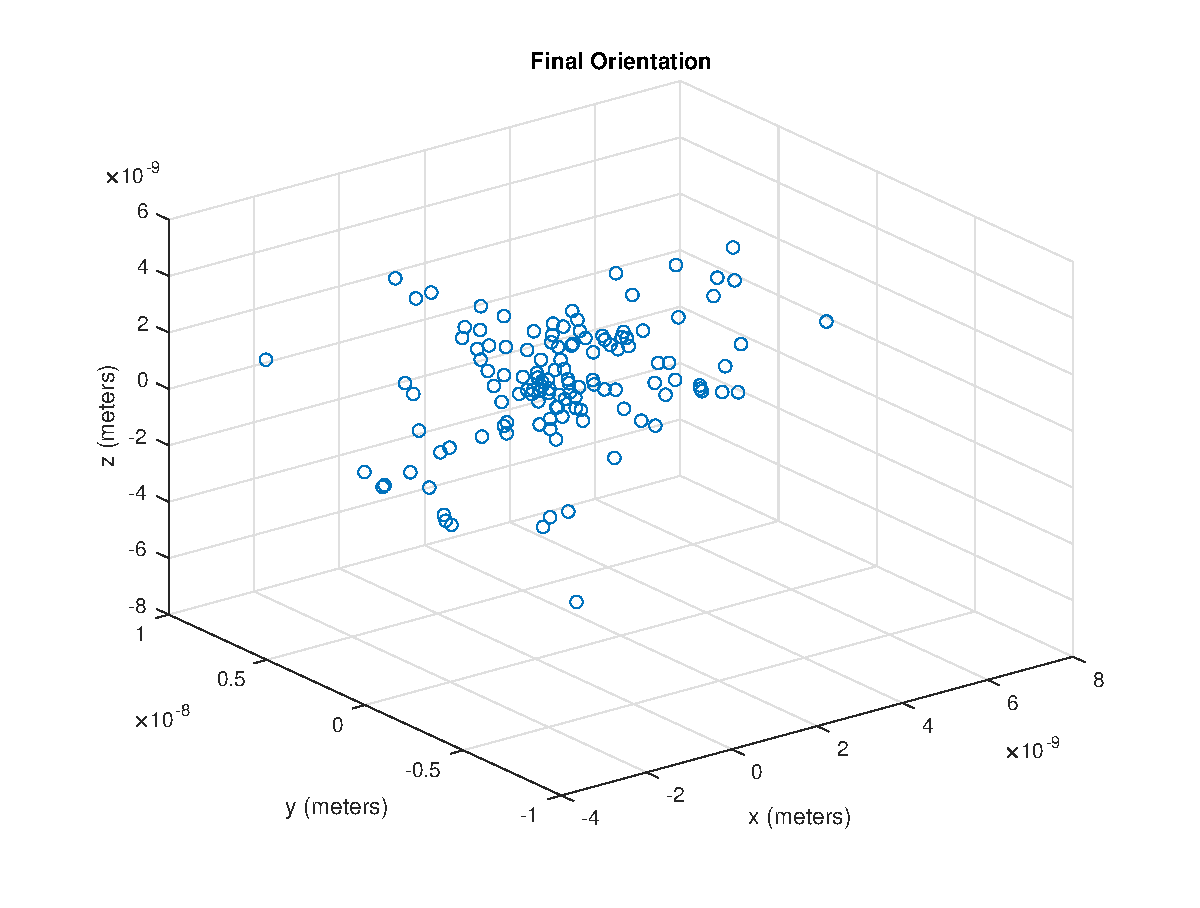
\includegraphics[width=\linewidth]{./finalpics/LJfinal1000.eps}
\caption{\label{LJfinal1000}}
\end{subfigure}
\begin{subfigure}{0.5\textwidth}
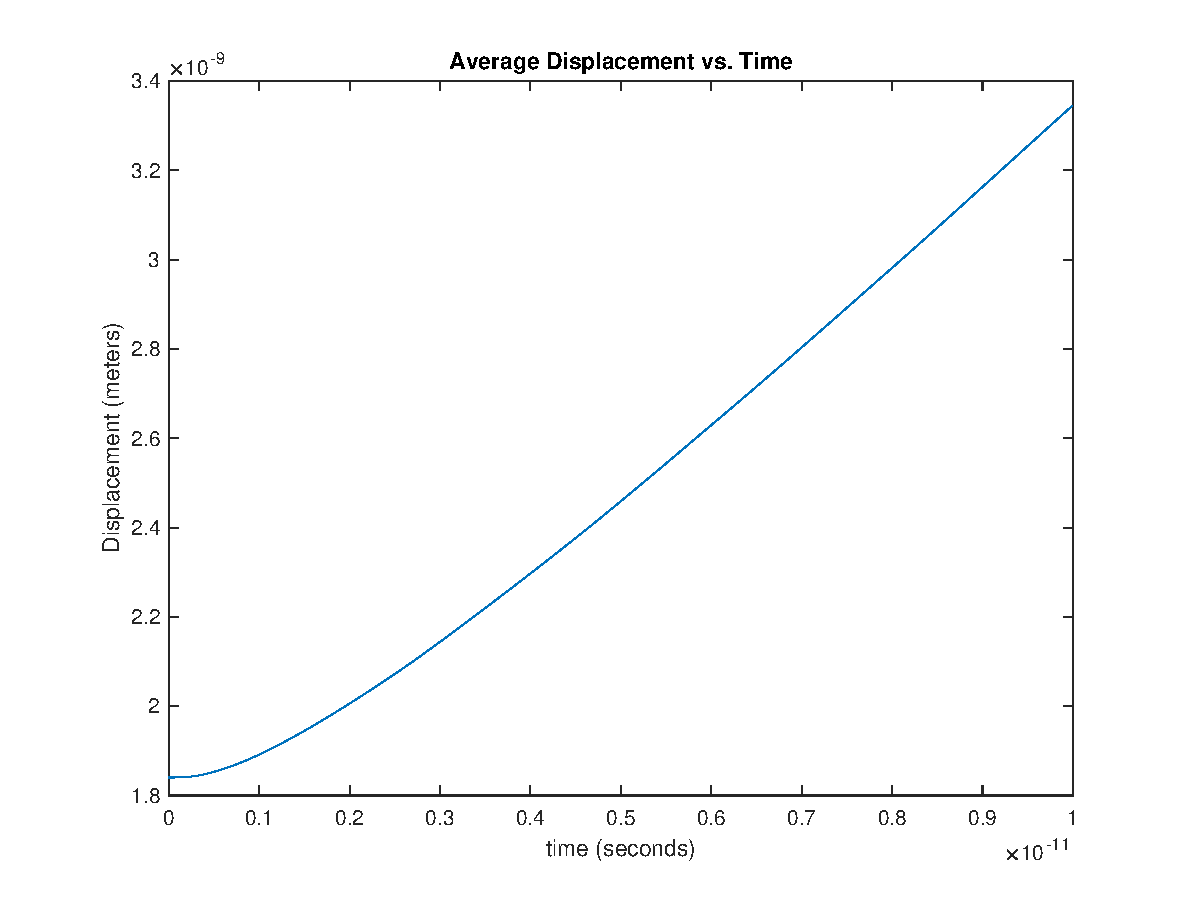
\includegraphics[width=\linewidth]{./finalpics/LJaverager1000.eps}
\caption{\label{LJaverage1000}}
\end{subfigure}
\caption{A 3D scatter plot of the final position (after $10^{-11}$ seconds) of a Xenon lattice in the Lennard-Jones potential (a) and the average magnitude of the displacement over time (b)  when initialized to 1000K.  It is clear from both plots the increased temperature causes more atoms to have enough energy to leave the initial lattice and evaporate.} 
\end{figure}

\begin{figure}[!h]
\begin{subfigure}{0.5\textwidth}
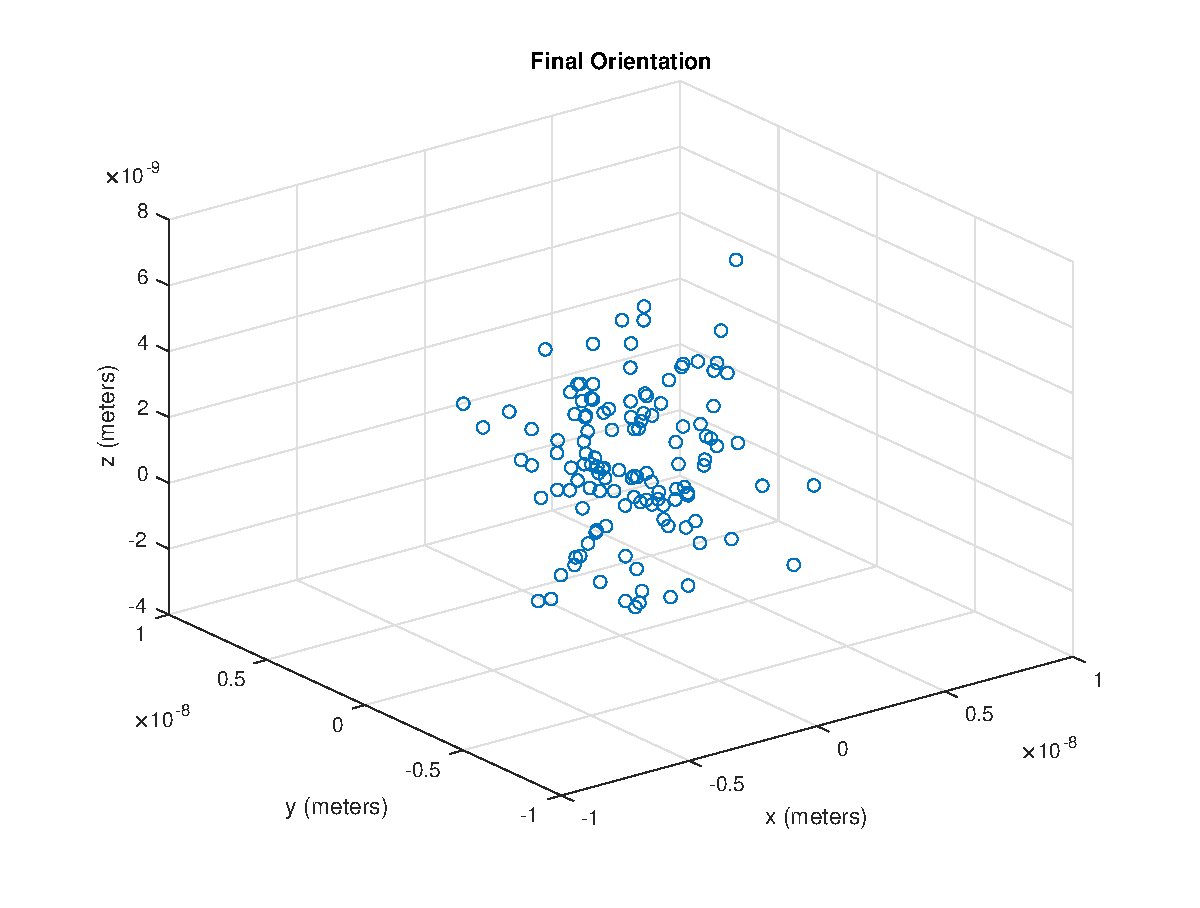
\includegraphics[width=\linewidth]{./finalpics/Mfinal1000.eps}
\caption{\label{mfinal1000}}
\end{subfigure}
\begin{subfigure}{0.5\textwidth}
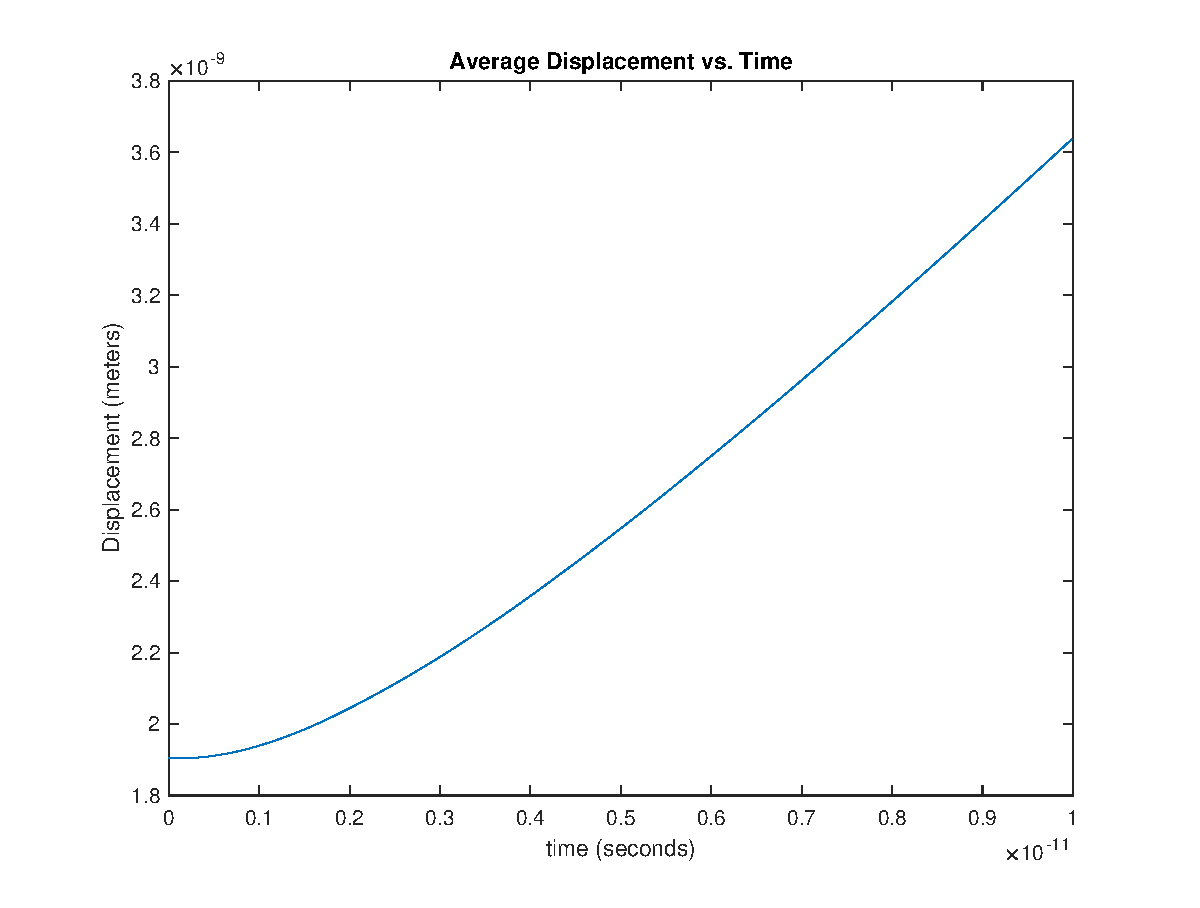
\includegraphics[width=\linewidth]{./finalpics/Maverager1000.eps}
\caption{\label{maverage1000}}
\end{subfigure}
\caption{A 3D scatter plot of the final position (after $10^{-11}$ seconds) of a Xenon lattice in the Morse potential (a) and the average magnitude of the displacement over time (b)  when initialized to 1000K.  It is clear from both plots the increased temperature causes more atoms to have enough energy to leave the system entirely and evaporate.} 
\end{figure}

Another noteworthy effect of temperature is the order that appears in the structure as temperature is lowered and the Xenon shifts from gas, to liquid, to solid.  To analyze this order, histograms of the final distance to neighbors in multiple simulations have been plotted in figs. \ref{LJrel}, \ref{LJrelhigh}, \ref{Mrel}, and \ref{Mrelhigh}.  The sharp peaks throughout at low temperatures is caused by the presence of long range order in the solid state of the material, and then as the temperature rises above the melting and boiling points, the peaks flatten and the long range order dissipates.  This follows naturally, as when the lattice is held at a lower temperature, it lacks the necessary kinetic energy to overcome the potential well and escape.  As it heats, some atoms have a higher probability of overcoming that well and evaporating.

\begin{figure}[!h]
\begin{subfigure}{0.5\textwidth}
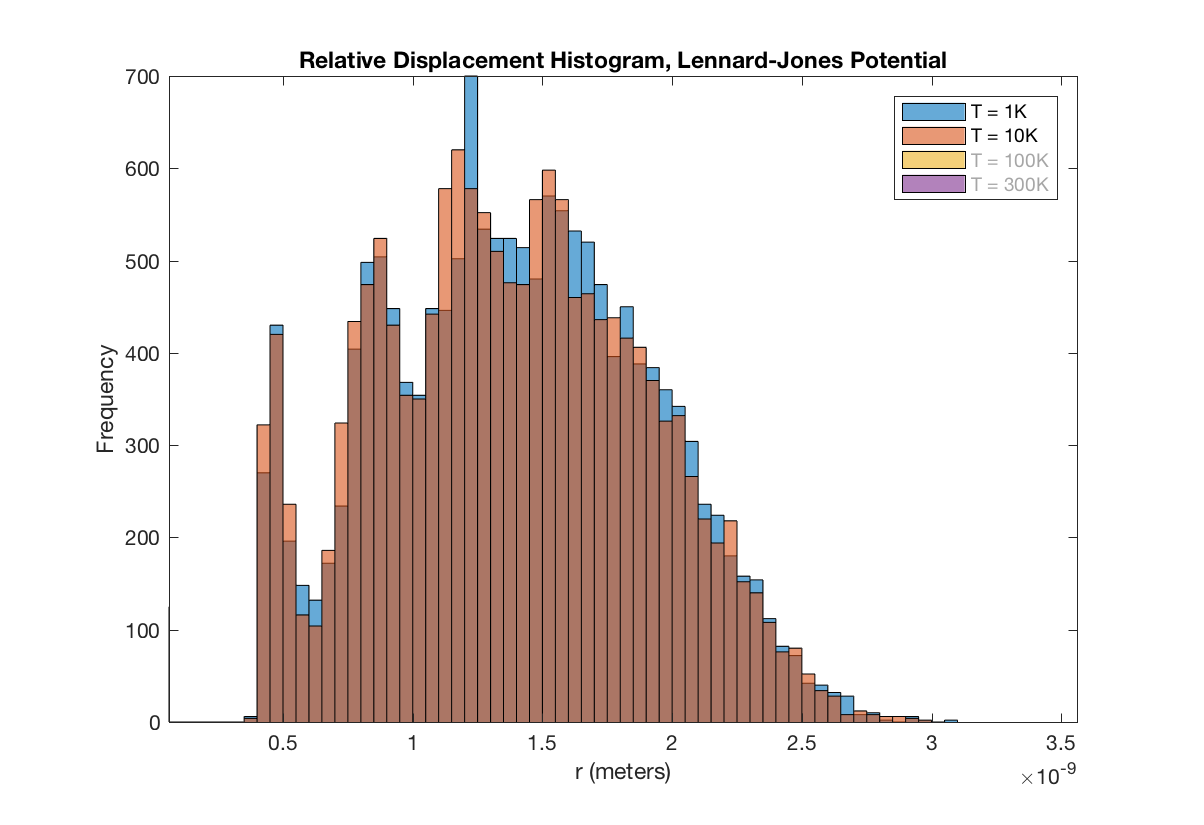
\includegraphics[width=0.9\linewidth]{./finalpics/LJfinalrelativer.eps}
\caption{\label{LJrel}}
\end{subfigure}
\begin{subfigure}{0.5\textwidth}
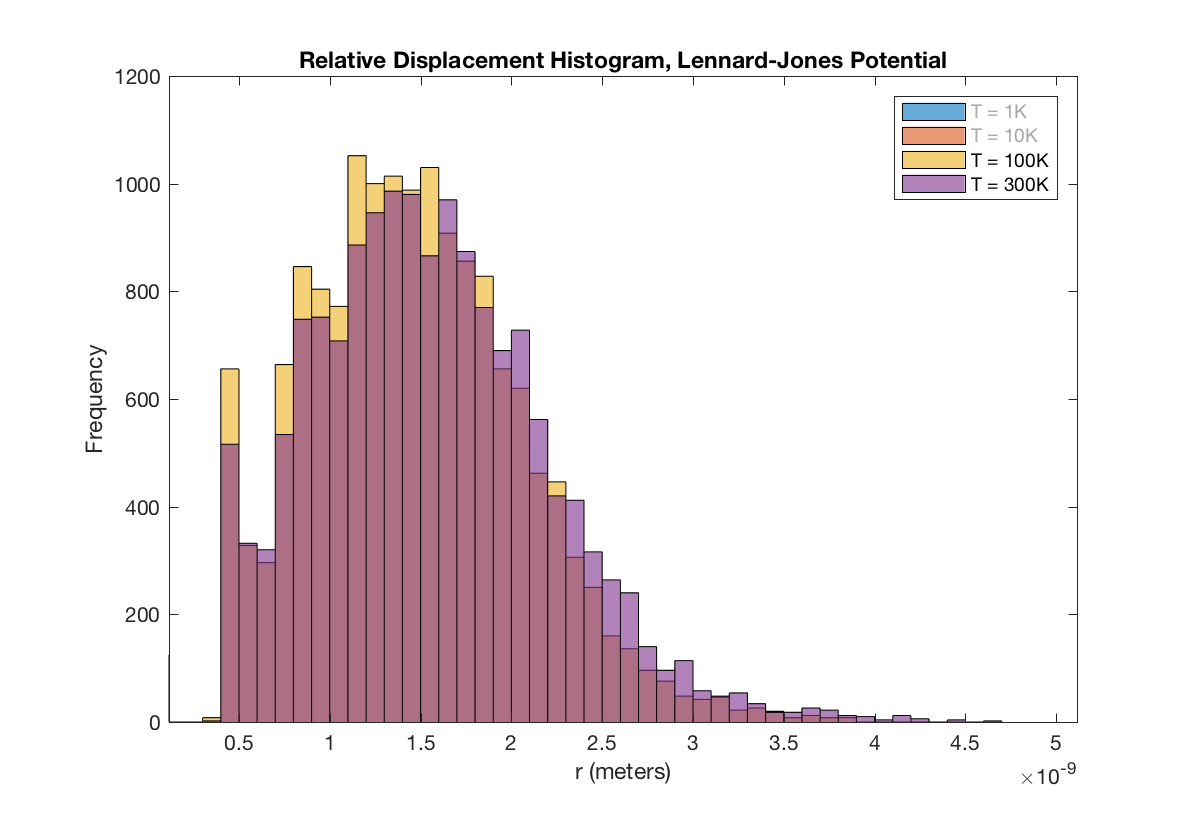
\includegraphics[width=0.9\linewidth]{./finalpics/LJfinalrelativerhighT.eps}
\caption{\label{LJrelhigh}}
\end{subfigure}
\caption{Histograms of the relative distance to all other particles in the system at (a) 1K and 10K, and (b) 100K and 300K in the Lennard-Jones potential.  Definite peaks occur at low temperatures across short and long range, and as the element transitions to liquid and gaseous phases, the long range order dissipates.} 
\end{figure}

\begin{figure}[!h]
\begin{subfigure}{0.5\textwidth}
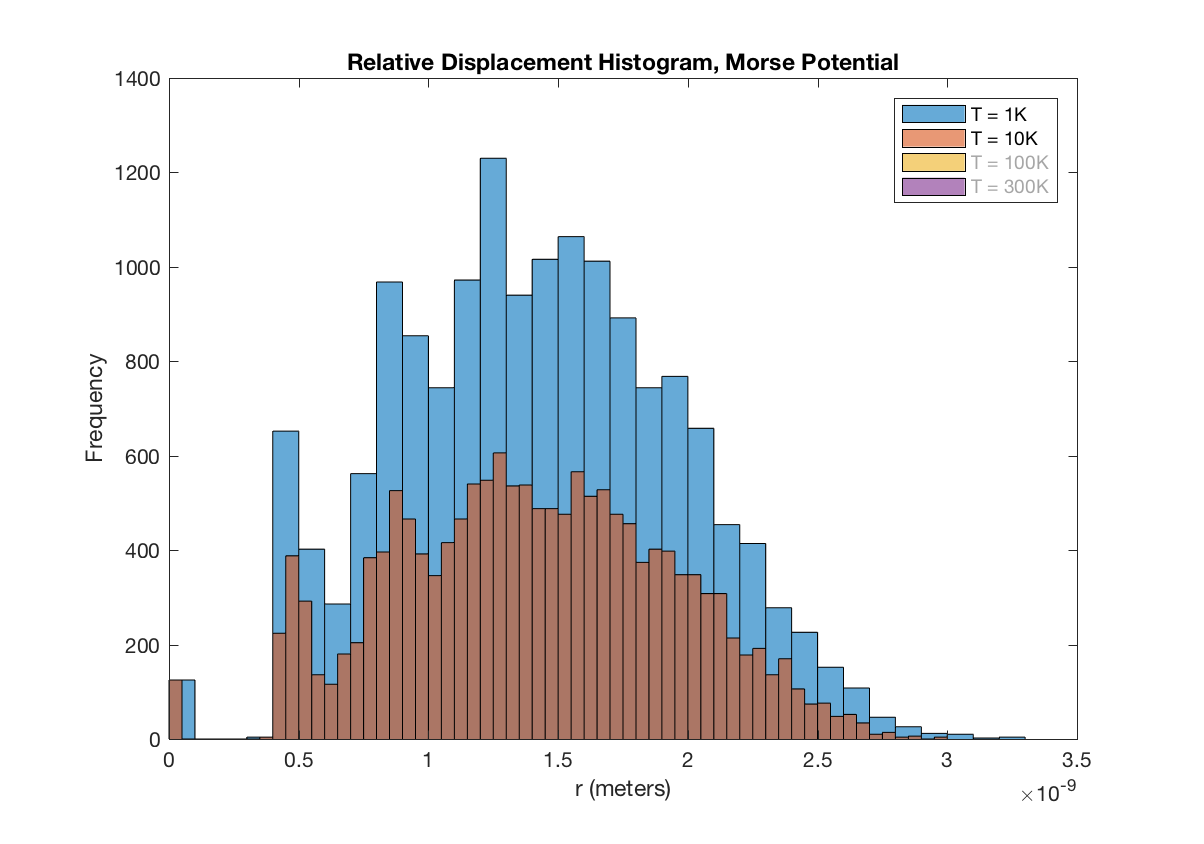
\includegraphics[width=0.9\linewidth]{./finalpics/Mfinalrelativer.eps}
\caption{\label{Mrel}}
\end{subfigure}
\begin{subfigure}{0.5\textwidth}
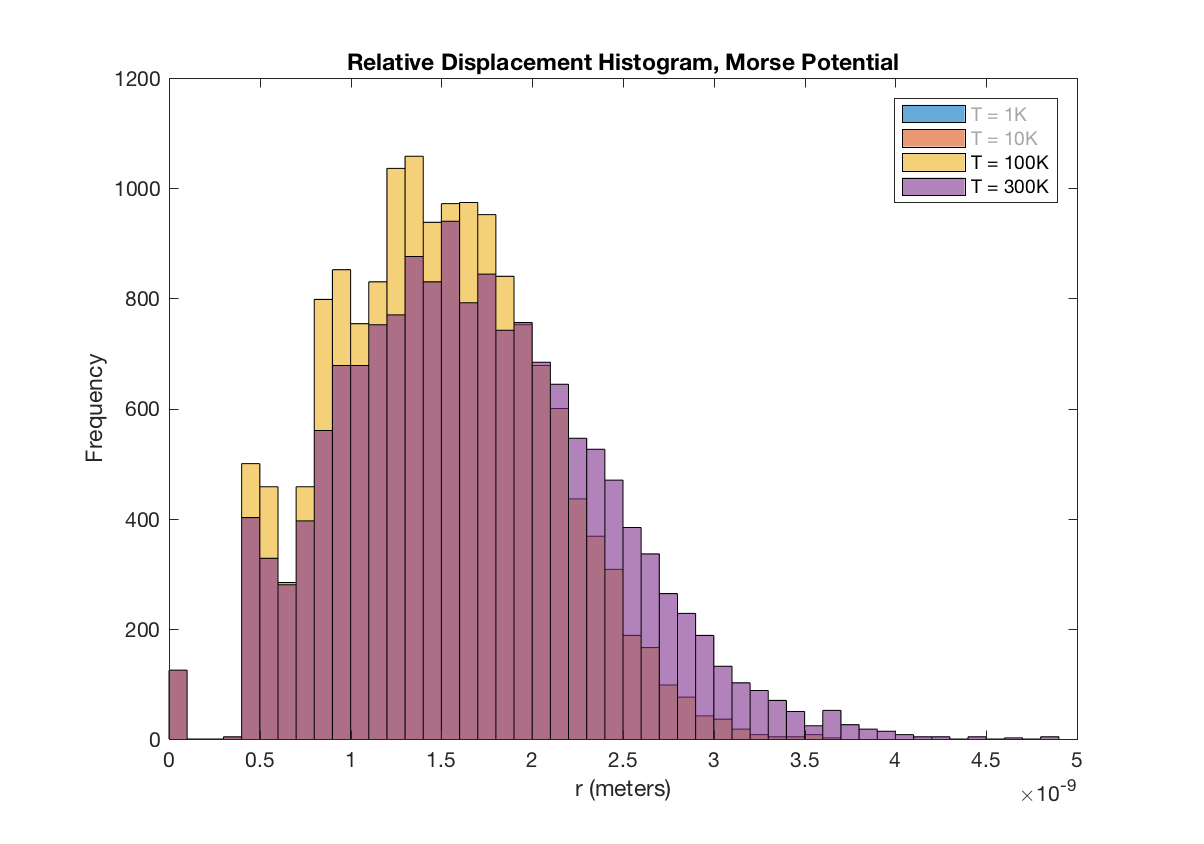
\includegraphics[width=0.9\linewidth]{./finalpics/MfinalrelativerhighT.eps}
\caption{\label{Mrelhigh}}
\end{subfigure}
\caption{Histograms of the relative distance to all other particles in the system at (a) 1K and 10K, and (b) 100K and 300K in the Lennard-Jones potential.  Definite peaks occur at low temperatures across short and long range, and as the element transitions to liquid and gaseous phases, the long range order dissipates.} 
\end{figure}

\section*{Conclusions}
The results of these simulations point to the viability of Verlet integration as a method of modeling the interactions between these atoms, provided an adequate time step.  This is proved by the conservation of energy and momentum within a variance of 0.01\%   Both the Lennard-Jones and Morse potentials are well-shaped potential curves that cause slight oscillatory behavior in the lattice, as seen in the expansion-contraction cycles in the simulation results. \cite{mpotential,ljpotential} The introduction of temperature variance in the lattice of Xenon atoms shows the transition between solid, liquid, and gas phases.  As temperature increases, more atoms evaporate, and the long range order evident in the solid dissipates.

\pagebreak
\section*{Acknowledgements}
I would like to thank Dr. Justin Oelgoetz for assistance formulating the simulation code, and for providing insightful explanations and troubleshooting along the way.

The ``random\_number" subroutine within the code was seeded using an algorithm provided by Justin Oelgoetz, as sourced from open source code online.  This code seeds Fortran's random number generator to create pseudo-random numbers that are unique to each run.

All graphs and plots made in this paper were produced using MATLAB computational software.
\newpage
\bibliographystyle{plain}
\bibliography{nbody}
\newpage
\section*{Appendix}
Attached is the source code for this project, written in Fortran.
\subsection*{Main}
\lstinputlisting[language=Fortran]{../nbody.f90}
\subsection*{Morse Potential Module}
\lstinputlisting[language=Fortran]{../morse.f90}
\subsection*{Lennard-Jones Potential Module}
\lstinputlisting[language=Fortran]{../lennardjones.f90}
\subsection*{Constants Module}
\lstinputlisting[language=Fortran]{../constants.f90}
\subsection*{MATLAB Plotting Script}
Code can be run while MATLAB is in the directory containing result files and will create a .gif file of positions, total energy and momentum plots, an initial velocity sampling histogram, average displacement magnitude vs. time, and initial and final scatter plots of position and save them to the directory.
\lstinputlisting[language=Octave]{../plots.m}
\end{document}